\documentclass[11pt,a4paper]{article}

% Packages
\usepackage[margin=2.5cm]{geometry}
\usepackage{microtype}
\usepackage{graphicx}
\usepackage{tikz}
\usetikzlibrary{shapes,arrows.meta,positioning,calc,fit,backgrounds,shadows.blur,decorations.pathmorphing,decorations.pathreplacing}
\usepackage{colortbl}
\usepackage{enumitem}
\usepackage{booktabs}
\usepackage{longtable}
\usepackage{hyperref}
\usepackage{xcolor}
\usepackage{fancyhdr}
\usepackage{titlesec}
\usepackage[most]{tcolorbox}
\usepackage{multicol}
\usepackage{amsmath,amssymb}
\usepackage{multirow}
\usepackage{setspace}
\usepackage{fontawesome5}
\usepackage{listings}

% Spacing
\setlength{\parskip}{3pt plus 1pt minus 1pt}
\setlength{\parindent}{0pt}

% Colors
\definecolor{primary}{HTML}{1A5276}
\definecolor{secondary}{HTML}{2E86C1}
\definecolor{accent}{HTML}{E74C3C}
\definecolor{lightbg}{HTML}{EBF5FB}
\definecolor{defbg}{HTML}{FDF2E9}
\definecolor{greenhl}{HTML}{27AE60}
\definecolor{purplehl}{HTML}{8E44AD}
\definecolor{codebg}{HTML}{F4F6F7}

% Hyperref
\hypersetup{colorlinks=true, linkcolor=primary, urlcolor=secondary, citecolor=primary}

% Code listings style
\lstset{
  backgroundcolor=\color{codebg},
  basicstyle=\ttfamily\small,
  keywordstyle=\color{primary}\bfseries,
  stringstyle=\color{greenhl},
  commentstyle=\color{gray},
  breaklines=true,
  frame=l,
  framerule=2pt,
  rulecolor=\color{secondary!40},
  xleftmargin=8pt,
  framexleftmargin=6pt,
  aboveskip=6pt,
  belowskip=6pt,
  showstringspaces=false,
  language=Python
}

% Header/Footer
\pagestyle{fancy}
\fancyhf{}
\fancyhead[L]{\small\textcolor{primary}{\textbf{Artificial Intelligence --- Core Concepts}}}
\fancyhead[R]{\small\textcolor{primary}{Lecture Handout}}
\fancyfoot[C]{\small\thepage}
\renewcommand{\headrulewidth}{0.5pt}
\renewcommand{\footrulewidth}{0.3pt}

% Section formatting
\titleformat{\section}{\Large\bfseries\color{primary}}{\thesection}{0.6em}{}[\vspace{2pt}\titlerule]
\titleformat{\subsection}{\large\bfseries\color{secondary}}{\thesubsection}{0.5em}{}
\titleformat{\subsubsection}{\normalsize\bfseries\color{primary}}{\thesubsubsection}{0.5em}{}
\titlespacing*{\section}{0pt}{14pt}{8pt}
\titlespacing*{\subsection}{0pt}{10pt}{5pt}

% Custom boxes
\newtcolorbox{definitionbox}[1][]{
  enhanced, breakable,
  colback=defbg, colframe=orange!60!black,
  colbacktitle=orange!70!black, coltitle=white,
  title={\faIcon{book}~#1}, fonttitle=\bfseries,
  boxrule=0pt, leftrule=4pt, arc=2pt,
  shadow={1mm}{-1mm}{0mm}{black!15},
  top=4pt, bottom=4pt, left=8pt, right=8pt
}
\newtcolorbox{conceptbox}[1][]{
  enhanced, breakable,
  colback=lightbg, colframe=secondary,
  colbacktitle=secondary, coltitle=white,
  title={\faIcon{lightbulb}~#1}, fonttitle=\bfseries,
  boxrule=0pt, leftrule=4pt, arc=2pt,
  shadow={1mm}{-1mm}{0mm}{black!15},
  top=4pt, bottom=4pt, left=8pt, right=8pt
}
\newtcolorbox{alertbox}[1][]{
  enhanced, breakable,
  colback=red!4, colframe=accent,
  colbacktitle=accent, coltitle=white,
  title={\faIcon{exclamation-triangle}~#1}, fonttitle=\bfseries,
  boxrule=0pt, leftrule=4pt, arc=2pt,
  shadow={1mm}{-1mm}{0mm}{black!12},
  top=3pt, bottom=3pt, left=8pt, right=8pt
}
\newtcolorbox{examplebox}[1][]{
  enhanced, breakable,
  colback=green!4, colframe=greenhl,
  colbacktitle=greenhl, coltitle=white,
  title={\faIcon{code}~#1}, fonttitle=\bfseries,
  boxrule=0pt, leftrule=4pt, arc=2pt,
  shadow={1mm}{-1mm}{0mm}{black!12},
  top=3pt, bottom=3pt, left=8pt, right=8pt
}

\begin{document}

% Title
\begin{center}
\vspace*{0.5cm}
{\Huge\bfseries\textcolor{primary}{Artificial Intelligence}}\\[8pt]
{\Huge\bfseries\textcolor{primary}{Core Concepts Handout}}\\[16pt]
{\color{secondary}\rule{0.68\textwidth}{1.5pt}}\\[14pt]
{\Large\textsc{Summer 2026 --- BSIT, 3rd Semester}}\\[8pt]
{\large\textcolor{gray!70!black}{Foundations $\bullet$ Agents $\bullet$ Search $\bullet$ Games $\bullet$ CSP $\bullet$ Planning $\bullet$ Knowledge $\bullet$ Learning $\bullet$ Ethics}}
\vspace{0.3cm}
\end{center}

\tableofcontents
\newpage

%=============================================================
\section{Introduction to Artificial Intelligence}
%=============================================================

\begin{definitionbox}[Artificial Intelligence]
Artificial Intelligence (AI) is the branch of computer science concerned with building systems that can \textbf{perceive}, \textbf{reason}, \textbf{learn}, and \textbf{act} to achieve goals, performing tasks that normally require human intelligence.
\end{definitionbox}

\begin{conceptbox}[Why AI Matters]
AI powers search engines, recommendation systems, voice assistants, self-driving cars, medical diagnosis tools, fraud detection, and chatbots. As a BSIT student, understanding AI fundamentals prepares you to design, use, and evaluate intelligent systems responsibly.
\end{conceptbox}

\subsection{A Brief History}
\begin{itemize}[leftmargin=*]
  \item \textbf{1950:} Alan Turing proposes the \emph{Turing Test} as a measure of machine intelligence.
  \item \textbf{1956:} The term ``Artificial Intelligence'' is coined at the Dartmouth Conference.
  \item \textbf{1980s:} Expert systems and rule-based AI become popular in industry.
  \item \textbf{1990s--2000s:} Machine learning and statistical approaches gain traction (e.g., IBM Deep Blue defeats a chess champion in 1997).
  \item \textbf{2010s--present:} Deep learning revolution --- image recognition, natural language processing, and generative AI (ChatGPT, GPT-4, and beyond).
\end{itemize}

\subsection{Approaches to AI}
\begin{center}
\begin{tikzpicture}[
  box/.style={rectangle, draw, thick, fill=#1, minimum width=3.0cm, minimum height=1.2cm, align=center, font=\small\bfseries, rounded corners=4pt,
    blur shadow={shadow blur steps=5, shadow xshift=0.5mm, shadow yshift=-0.5mm}},
  arr/.style={-{Stealth}, thick, primary!60}
]
  \node[box=primary!15] (ai) at (0,0) {\faIcon{robot}\\Artificial\\Intelligence};
  \node[box=blue!12] (rule) at (-5.5,-2.3) {\faIcon{list-ol}\\Rule-Based /\\Symbolic AI};
  \node[box=orange!12] (ml) at (0,-2.3) {\faIcon{brain}\\Machine\\Learning};
  \node[box=green!12] (dl) at (5.5,-2.3) {\faIcon{network-wired}\\Deep\\Learning};
  \draw[arr] (ai) -- (rule);
  \draw[arr] (ai) -- (ml);
  \draw[arr] (ai) -- (dl);
\end{tikzpicture}
\end{center}
\begin{itemize}[leftmargin=*]
  \item \textbf{Rule-Based (Symbolic) AI:} Explicit if--then rules and logic written by humans (expert systems).
  \item \textbf{Machine Learning:} Systems learn patterns automatically from data instead of hard-coded rules.
  \item \textbf{Deep Learning:} A subset of ML using multi-layer neural networks for complex tasks like vision and language.
\end{itemize}

\subsection{Types of AI by Capability}
\begin{itemize}[leftmargin=*]
  \item \textbf{Narrow AI (Weak AI):} Designed for a specific task (spam filters, recommendation engines, voice assistants). All AI in use today is narrow AI.
  \item \textbf{General AI (Strong AI):} A hypothetical system with human-level intelligence across all tasks. Does not yet exist.
  \item \textbf{Super AI:} A hypothetical AI surpassing human intelligence in all domains. Purely theoretical.
\end{itemize}

%=============================================================
\section{Intelligent Agents}
%=============================================================

\begin{definitionbox}[Intelligent Agent]
An intelligent agent \textbf{perceives} its environment through sensors and \textbf{acts} upon it through actuators to achieve goals, following an \emph{agent function} that maps percepts to actions.
\end{definitionbox}

\begin{center}
\begin{tikzpicture}[
  box/.style={rectangle, draw, thick, fill=#1, minimum width=2.8cm, minimum height=1.2cm, align=center, font=\small\bfseries, rounded corners=4pt,
    blur shadow={shadow blur steps=5, shadow xshift=0.5mm, shadow yshift=-0.5mm}},
  arr/.style={-{Stealth[length=3mm]}, very thick, line width=1.5pt}
]
  \node[box=blue!15] (agent) at (0,0) {\faIcon{user-cog}\\Agent};
  \node[box=green!15] (env) at (7,0) {\faIcon{globe}\\Environment};
  \draw[arr, primary!70] (agent.north east) -- node[above, font=\small] {Actions (actuators)} (env.north west);
  \draw[arr, greenhl!70] (env.south west) -- node[below, font=\small] {Percepts (sensors)} (agent.south east);
\end{tikzpicture}
\end{center}

\subsection{Types of Agents}
\begin{itemize}[leftmargin=*]
  \item \textbf{Simple Reflex Agents:} Act only on the current percept using condition--action rules (e.g., a thermostat).
  \item \textbf{Model-Based Reflex Agents:} Maintain an internal state to track aspects of the world not directly observed.
  \item \textbf{Goal-Based Agents:} Choose actions that help achieve an explicit goal, considering future consequences.
  \item \textbf{Utility-Based Agents:} Choose actions that maximize a utility function, allowing trade-offs between competing goals.
  \item \textbf{Learning Agents:} Improve performance over time using feedback from a performance element and a learning element.
\end{itemize}

\subsection{Properties of Task Environments (PEAS)}
\rowcolors{2}{white}{defbg}
\begin{longtable}{@{}p{2.2cm}p{11.3cm}@{}}
\toprule
\rowcolor{primary!15}
\textbf{PEAS} & \textbf{Description} \\
\midrule
\endhead
Performance measure & Criteria for success (e.g., accuracy, speed, safety). \\
\addlinespace
Environment & The surroundings the agent operates in (e.g., roads, chessboard, web). \\
\addlinespace
Actuators & Mechanisms the agent uses to act (e.g., wheels, screen, robotic arm). \\
\addlinespace
Sensors & Mechanisms the agent uses to perceive (e.g., camera, microphone, keyboard). \\
\bottomrule
\end{longtable}

%=============================================================
\section{Problem Solving by Search}
%=============================================================

\begin{definitionbox}[Search Problem]
A search problem consists of an \textbf{initial state}, a set of \textbf{actions}, a \textbf{transition model}, a \textbf{goal test}, and a \textbf{path cost} function. Solving it means finding a sequence of actions from the initial state to a goal state.
\end{definitionbox}

\subsection{Uninformed (Blind) Search}
\begin{itemize}[leftmargin=*]
  \item \textbf{Breadth-First Search (BFS):} Explores all nodes at the current depth before moving deeper; guarantees the shallowest solution.
  \item \textbf{Depth-First Search (DFS):} Explores as far as possible along a branch before backtracking; memory-efficient but not always optimal.
  \item \textbf{Uniform Cost Search:} Expands the node with the lowest path cost so far; optimal for weighted graphs.
  \item \textbf{Iterative Deepening DFS (IDDFS):} Repeats DFS with increasing depth limits ($0, 1, 2, \ldots$); combines BFS's completeness with DFS's low memory use.
  \item \textbf{Bidirectional Search:} Simultaneously searches forward from the initial state and backward from the goal, meeting in the middle to cut the effective search depth.
\end{itemize}

\subsection{Informed (Heuristic) Search}
\begin{definitionbox}[Heuristic Function]
A heuristic $h(n)$ estimates the cost from node $n$ to the nearest goal, guiding the search toward promising paths without exploring the entire space.
\end{definitionbox}
\begin{itemize}[leftmargin=*]
  \item \textbf{Greedy Best-First Search:} Expands the node that appears closest to the goal using $h(n)$ only; fast but not always optimal.
  \item \textbf{A* Search:} Expands the node with the lowest $f(n) = g(n) + h(n)$, where $g(n)$ is the cost so far; optimal when $h(n)$ is admissible (never overestimates).
\end{itemize}

\subsection{Search Strategy Comparison}
\rowcolors{2}{white}{defbg}
\begin{longtable}{@{}p{2.7cm}p{2.2cm}p{2.2cm}p{2.2cm}p{4.0cm}@{}}
\toprule
\rowcolor{primary!15}
\textbf{Algorithm} & \textbf{Complete} & \textbf{Optimal} & \textbf{Memory} & \textbf{Notes} \\
\midrule
\endhead
BFS & Yes & Yes (unit step cost) & High & Good for shallow solutions; can explode in memory. \\
\addlinespace
DFS & No (in infinite trees) & No & Low & Fast memory-wise but may get trapped in deep branches. \\
\addlinespace
Uniform Cost & Yes & Yes & High & Best when step costs differ. \\
\addlinespace
Iterative Deepening & Yes & Yes (unit step cost) & Low & Combines BFS's completeness with DFS's memory efficiency. \\
\addlinespace
Bidirectional & Yes (conditions apply) & Yes (conditions apply) & Medium & Needs a well-defined goal and reversible actions; can greatly cut search time. \\
\addlinespace
Greedy Best-First & No & No & Medium & Often fast, but can take wrong shortcuts. \\
\addlinespace
A* & Yes & Yes (admissible $h$) & High & Practical and widely used in pathfinding. \\
\bottomrule
\end{longtable}

\subsection{Worked Search Example}
\begin{examplebox}[A* in One Minute]
Suppose a robot starts at node $S$ and wants to reach goal $G$. For each frontier node, A* computes:
$$f(n)=g(n)+h(n)$$
where $g(n)$ is the cost from $S$ to $n$, and $h(n)$ is estimated cost from $n$ to $G$.
If frontier values are $A:(g=2,h=5,f=7)$, $B:(g=4,h=2,f=6)$, and $C:(g=3,h=4,f=7)$, A* chooses $B$ first because it has the minimum $f$. This process repeats until the goal is selected.
\end{examplebox}

\subsection{Local Search and Optimization}
\begin{itemize}[leftmargin=*]
  \item \textbf{Hill Climbing:} Moves to the neighboring state with the best value; can get stuck at local maxima.
  \item \textbf{Simulated Annealing:} Allows occasional ``worse'' moves to escape local maxima, with randomness decreasing over time.
  \item \textbf{Genetic Algorithms:} Maintain a population of candidate solutions that evolve via selection, crossover, and mutation.
\end{itemize}

%=============================================================
\section{Adversarial Search and Game Playing}
%=============================================================

\begin{definitionbox}[Adversarial Search]
Adversarial search handles environments with two or more competing agents, such as chess or tic-tac-toe. Each player chooses moves that best serve its own interest while anticipating the opponent's best response.
\end{definitionbox}

\subsection{The Minimax Algorithm}
\begin{definitionbox}[Minimax]
Minimax explores the game tree assuming the \textbf{MAX} player always picks the move with the highest value and the \textbf{MIN} player always picks the move with the lowest value. Values are ``backed up'' from the leaves toward the root.
\end{definitionbox}

\begin{center}
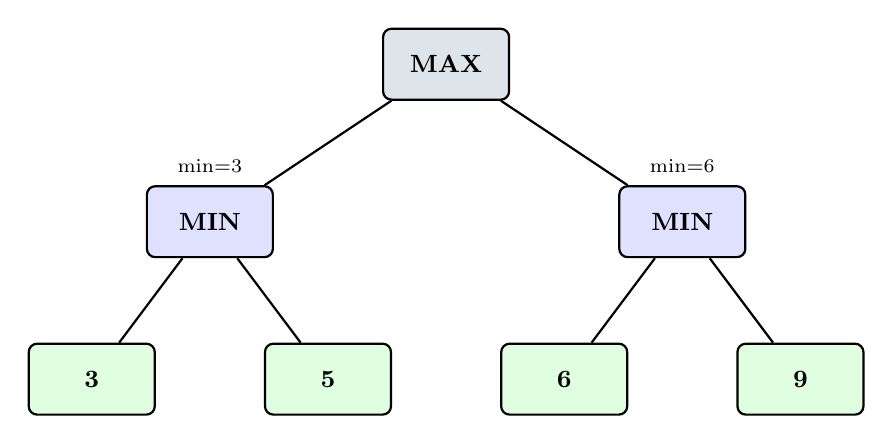
\begin{tikzpicture}[
  gbox/.style={rectangle, draw, thick, fill=#1, minimum width=1.6cm, minimum height=0.9cm, align=center, font=\small\bfseries, rounded corners=3pt}
]
  \node[gbox=primary!15] (root) at (0,0) {MAX};
  \node[gbox=blue!12] (m1) at (-3,-2) {MIN};
  \node[gbox=blue!12] (m2) at (3,-2) {MIN};
  \node[gbox=green!12] (l1) at (-4.5,-4) {3};
  \node[gbox=green!12] (l2) at (-1.5,-4) {5};
  \node[gbox=green!12] (l3) at (1.5,-4) {6};
  \node[gbox=green!12] (l4) at (4.5,-4) {9};
  \draw[thick] (root) -- (m1);
  \draw[thick] (root) -- (m2);
  \draw[thick] (m1) -- (l1);
  \draw[thick] (m1) -- (l2);
  \draw[thick] (m2) -- (l3);
  \draw[thick] (m2) -- (l4);
  \node[font=\scriptsize, above=1pt of m1] {min=3};
  \node[font=\scriptsize, above=1pt of m2] {min=6};
\end{tikzpicture}
\end{center}

\subsection{Alpha-Beta Pruning}
\begin{conceptbox}[Alpha-Beta Pruning]
Alpha-beta pruning speeds up minimax by skipping branches that cannot change the final decision. It tracks $\alpha$ (best value MAX can guarantee so far) and $\beta$ (best value MIN can guarantee so far); a branch is pruned whenever $\alpha \geq \beta$.
\end{conceptbox}
\begin{itemize}[leftmargin=*]
  \item Produces the \textbf{same decision} as plain minimax, but explores fewer nodes.
  \item Best case reduces complexity from $O(b^d)$ to $O(b^{d/2})$, where $b$ is the branching factor and $d$ is the depth.
  \item Exploring the best moves first increases the amount of pruning achieved.
\end{itemize}

\begin{examplebox}[Worked Example: Minimax Backed-Up Values]
Given leaf values $3, 5, 6, 9$ (left to right, as in the diagram above):
\begin{itemize}[leftmargin=*]
  \item Left MIN node: $\min(3,5)=3$
  \item Right MIN node: $\min(6,9)=6$
  \item Root MAX node: $\max(3,6)=6$
\end{itemize}
MAX should choose the move leading to the right subtree, guaranteeing a value of \textbf{6}.
\end{examplebox}

%=============================================================
\section{Constraint Satisfaction Problems (CSP)}
%=============================================================

\begin{definitionbox}[Constraint Satisfaction Problem]
A CSP consists of a set of \textbf{variables}, a \textbf{domain} of possible values for each variable, and a set of \textbf{constraints} restricting which value combinations are allowed. A solution assigns a value to every variable while satisfying all constraints.
\end{definitionbox}

\subsection{Common CSP Examples}
\begin{itemize}[leftmargin=*]
  \item \textbf{Map Coloring:} Color regions so that no two adjacent regions share a color.
  \item \textbf{Sudoku:} Fill digits 1--9 so rows, columns, and boxes have no repeats.
  \item \textbf{N-Queens:} Place $N$ queens on a board so that none attacks another.
  \item \textbf{Timetabling:} Assign time slots to classes without room or teacher conflicts.
\end{itemize}

\subsection{Solving Techniques}
\begin{itemize}[leftmargin=*]
  \item \textbf{Backtracking Search:} Assigns variables one at a time and undoes an assignment when it violates a constraint.
  \item \textbf{Forward Checking:} Removes now-invalid values from neighboring domains immediately after each assignment.
  \item \textbf{Constraint Propagation:} Enforces arc consistency so every remaining value stays compatible with related variables.
  \item \textbf{Variable/Value Ordering Heuristics:} Minimum Remaining Values (MRV), Degree Heuristic, and Least Constraining Value guide which variable/value to try next.
\end{itemize}

\begin{center}
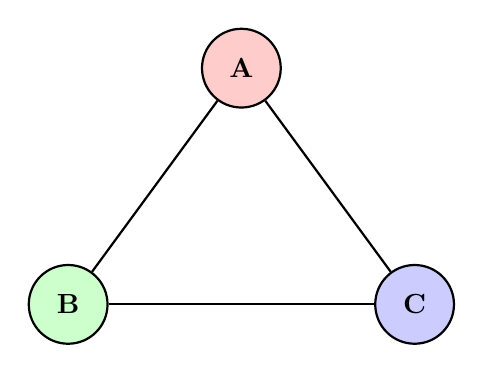
\begin{tikzpicture}
  \node[circle, draw, thick, fill=red!20, minimum size=1cm, font=\bfseries] (A) at (0,2) {A};
  \node[circle, draw, thick, fill=green!20, minimum size=1cm, font=\bfseries] (B) at (-2.2,-1) {B};
  \node[circle, draw, thick, fill=blue!20, minimum size=1cm, font=\bfseries] (C) at (2.2,-1) {C};
  \draw[thick] (A) -- (B);
  \draw[thick] (B) -- (C);
  \draw[thick] (C) -- (A);
\end{tikzpicture}
\end{center}

\begin{examplebox}[Worked Example: Map Coloring]
Regions $A$, $B$, and $C$ are mutually adjacent; available colors are \{Red, Green, Blue\}.
\begin{itemize}[leftmargin=*]
  \item Assign $A=$ Red.
  \item $B$ is adjacent to $A$, so $B \neq$ Red $\Rightarrow$ assign $B=$ Green.
  \item $C$ is adjacent to both $A$ and $B$, so $C \neq$ Red, Green $\Rightarrow$ assign $C=$ Blue.
\end{itemize}
All constraints are satisfied on the first attempt --- no backtracking was needed.
\end{examplebox}

%=============================================================
\section{Planning in AI}
%=============================================================

\begin{definitionbox}[Planning]
Planning is the AI task of finding a sequence of actions that transforms an initial state into a goal state, where each action is described by its \textbf{preconditions} (what must be true to apply it) and \textbf{effects} (what becomes true afterward).
\end{definitionbox}

\subsection{The STRIPS Representation}
\begin{conceptbox}[STRIPS]
STRIPS (STanford Research Institute Problem Solver) represents each planning action using three components:
\begin{itemize}[leftmargin=*]
  \item \textbf{Precondition:} Facts that must hold before the action can be executed.
  \item \textbf{Add List:} Facts that become true after the action.
  \item \textbf{Delete List:} Facts that become false after the action.
\end{itemize}
\end{conceptbox}

\subsection{Forward vs.\ Backward Planning}
\begin{itemize}[leftmargin=*]
  \item \textbf{Forward (Progression) Planning:} Searches forward from the initial state, applying actions whose preconditions are satisfied, until the goal is reached.
  \item \textbf{Backward (Regression) Planning:} Searches backward from the goal, selecting actions whose effects satisfy part of the goal, until the initial state is reached.
\end{itemize}

\begin{examplebox}[Worked Example: A Simple Plan]
Goal: \textit{Have a cup of tea}. Action \textsc{BoilWater}: precondition \{Kettle Filled\}, effect \{Water Boiled\}. Action \textsc{MakeTea}: precondition \{Water Boiled\}, effect \{Tea Ready\}.
\begin{itemize}[leftmargin=*]
  \item Start: \{Kettle Filled\}
  \item Apply \textsc{BoilWater} $\to$ \{Kettle Filled, Water Boiled\}
  \item Apply \textsc{MakeTea} $\to$ \{Kettle Filled, Water Boiled, Tea Ready\} --- \textbf{goal reached}
\end{itemize}
Plan found: $\langle \textsc{BoilWater}, \textsc{MakeTea} \rangle$.
\end{examplebox}

%=============================================================
\section{Knowledge Representation and Reasoning}
%=============================================================

\begin{definitionbox}[Knowledge Representation]
Knowledge representation is how an AI system encodes facts about the world so it can reason, draw conclusions, and make decisions.
\end{definitionbox}

\subsection{Logic-Based Representation}
\begin{itemize}[leftmargin=*]
  \item \textbf{Propositional Logic:} Statements that are either true or false, combined using AND ($\land$), OR ($\lor$), NOT ($\lnot$), and IMPLIES ($\Rightarrow$).
  \item \textbf{First-Order Logic:} Extends propositional logic with objects, relations, and quantifiers ($\forall$, $\exists$) for richer expressiveness.
  \item \textbf{Inference:} Deriving new facts from known facts using rules such as \emph{Modus Ponens}: from $P$ and $P \Rightarrow Q$, conclude $Q$.
\end{itemize}

\subsection{Rule-Based Expert Systems}
\begin{conceptbox}[Expert System]
An expert system uses a \textbf{knowledge base} of if--then rules and an \textbf{inference engine} to mimic the decision-making of a human expert in a specific domain (e.g., medical diagnosis, loan approval).
\end{conceptbox}

\subsection{Semantic Networks and Frames}
\begin{itemize}[leftmargin=*]
  \item \textbf{Semantic Network:} A graph of nodes (objects/concepts) connected by labeled edges representing relationships (e.g., ``Bird'' --\textit{is-a}--> ``Animal'').
  \item \textbf{Frames:} Structured representations that group an object's attributes (\textit{slots}) and their values, similar to a record or object in programming.
  \item \textbf{Ontology:} A formal, shared vocabulary of concepts and relationships within a domain, enabling knowledge reuse and reasoning across systems.
\end{itemize}

\subsection{Forward Chaining vs.\ Backward Chaining}
\begin{itemize}[leftmargin=*]
  \item \textbf{Forward Chaining (data-driven):} Starts from known facts and repeatedly applies rules to derive new facts until the goal is reached. Common in monitoring and planning systems.
  \item \textbf{Backward Chaining (goal-driven):} Starts from the goal and works backward, checking which rules could conclude it and recursively verifying their conditions. Common in diagnosis and query-answering systems (e.g., Prolog).
\end{itemize}

\begin{examplebox}[Worked Example: Forward Chaining]
Rules: (1) If \textit{it has feathers} $\Rightarrow$ \textit{it is a bird}. (2) If \textit{it is a bird} $\Rightarrow$ \textit{it can fly}.\\
Fact: \textit{Tweety has feathers}.\\
Forward chaining: feathers $\Rightarrow$ bird (Rule 1) $\Rightarrow$ can fly (Rule 2). Conclusion: \textbf{Tweety can fly.}
\end{examplebox}

%=============================================================
\section{Reasoning Under Uncertainty}
%=============================================================

\begin{definitionbox}[Why Uncertainty?]
Real-world knowledge is often incomplete or imprecise. AI systems use probability and fuzzy methods to reason sensibly despite uncertainty, instead of requiring rigid true/false facts.
\end{definitionbox}

\subsection{Bayesian Networks}
\begin{conceptbox}[Bayesian Network]
A Bayesian network is a directed acyclic graph where nodes represent random variables and edges represent probabilistic dependencies. Each node stores a conditional probability table (CPT) given its parents, and Bayes' theorem is used to update beliefs as new evidence arrives.
\end{conceptbox}

\subsection{Fuzzy Logic}
\begin{definitionbox}[Fuzzy Logic]
Fuzzy logic allows truth values between 0 and 1 (partial truth) instead of strict true/false, modeling vague concepts such as ``hot'', ``fast'', or ``tall'' using \textbf{membership functions}.
\end{definitionbox}
\begin{itemize}[leftmargin=*]
  \item \textbf{Crisp Set:} An element either belongs (1) or does not belong (0) to a set.
  \item \textbf{Fuzzy Set:} An element has a \textbf{degree of membership} $\mu(x) \in [0,1]$ (e.g., a temperature of $28^{\circ}$C might have $\mu_{\text{hot}}=0.7$).
  \item \textbf{Applications:} Washing machines, air conditioners, anti-lock braking systems, and other control systems requiring smooth decision boundaries.
\end{itemize}

%=============================================================
\section{Machine Learning Fundamentals}
%=============================================================

\begin{definitionbox}[Machine Learning]
Machine learning is a subset of AI in which systems \textbf{learn patterns from data} rather than following explicitly programmed rules, improving performance on a task through experience.
\end{definitionbox}

\subsection{Main Categories}
\begin{center}
\begin{tikzpicture}[
  box/.style={rectangle, draw, thick, fill=#1, minimum width=3.0cm, minimum height=1.1cm, align=center, font=\small\bfseries, rounded corners=4pt,
    blur shadow={shadow blur steps=5, shadow xshift=0.5mm, shadow yshift=-0.5mm}},
  arr/.style={-{Stealth}, thick, primary!60}
]
  \node[box=primary!15] (ml) at (0,0) {\faIcon{brain}\\Machine Learning};
  \node[box=blue!12] (sup) at (-5.2,-2.3) {\faIcon{chalkboard-teacher}\\Supervised};
  \node[box=orange!12] (unsup) at (0,-2.3) {\faIcon{search}\\Unsupervised};
  \node[box=green!12] (rl) at (5.2,-2.3) {\faIcon{gamepad}\\Reinforcement};
  \draw[arr] (ml) -- (sup);
  \draw[arr] (ml) -- (unsup);
  \draw[arr] (ml) -- (rl);
\end{tikzpicture}
\end{center}
\begin{itemize}[leftmargin=*]
  \item \textbf{Supervised Learning:} Learns from labeled input-output pairs (classification, regression).
  \item \textbf{Unsupervised Learning:} Finds hidden patterns in unlabeled data (clustering, dimensionality reduction).
  \item \textbf{Reinforcement Learning:} Learns by trial and error, receiving rewards or penalties from the environment.
\end{itemize}

\subsection{The ML Workflow}
\begin{center}
\begin{tikzpicture}[
  step/.style={rectangle, draw, thick, fill=#1, minimum width=2.1cm, minimum height=1.3cm, align=center, font=\footnotesize\bfseries, rounded corners=4pt,
    blur shadow={shadow blur steps=5, shadow xshift=0.5mm, shadow yshift=-0.5mm}},
  arr/.style={-{Stealth[length=2.5mm]}, very thick, primary!60, line width=1.2pt}
]
  \node[step=blue!12]   (s1) at (0,0)    {\faIcon{database}\\Collect\\Data};
  \node[step=cyan!12]   (s2) at (2.7,0)  {\faIcon{broom}\\Clean\\Data};
  \node[step=orange!12] (s3) at (5.4,0)  {\faIcon{cogs}\\Feature\\Engineering};
  \node[step=yellow!15] (s4) at (8.1,0)  {\faIcon{brain}\\Train\\Model};
  \node[step=green!12]  (s5) at (10.8,0) {\faIcon{chart-bar}\\Evaluate};
  \draw[arr] (s1) -- (s2);
  \draw[arr] (s2) -- (s3);
  \draw[arr] (s3) -- (s4);
  \draw[arr] (s4) -- (s5);
\end{tikzpicture}
\end{center}

\subsection{Core Supervised Learning Algorithms}
\begin{itemize}[leftmargin=*]
  \item \textbf{Linear Regression:} Fits a straight line $\hat{y}=w_0+w_1x$ to predict continuous values by minimizing mean squared error.
  \item \textbf{Logistic Regression:} Uses the sigmoid function $\sigma(z)=\frac{1}{1+e^{-z}}$ to output a probability for binary classification.
  \item \textbf{Decision Trees:} Split data recursively using the feature that gives the highest \textbf{information gain} (based on entropy), forming a tree of if--then decisions.
  \item \textbf{K-Nearest Neighbors (KNN):} Classifies a new point by majority vote among its $k$ closest labeled points, using a distance metric (e.g., Euclidean distance).
  \item \textbf{Naive Bayes:} Applies Bayes' theorem assuming features are conditionally independent given the class:
  $$
  P(\text{class}|\text{features}) \propto P(\text{class})\prod_i P(\text{feature}_i|\text{class})
  $$
  \item \textbf{Support Vector Machines (SVM):} Finds the hyperplane that separates classes with the \textbf{maximum margin} between the closest points (support vectors).
\end{itemize}

\subsection{Core Unsupervised Learning Algorithms}
\begin{itemize}[leftmargin=*]
  \item \textbf{K-Means Clustering:} Partitions data into $k$ clusters by repeating two steps: (1) assign each point to the nearest centroid, (2) recompute each centroid as the mean of its assigned points, until convergence.
  \item \textbf{Hierarchical Clustering:} Builds a tree (dendrogram) of nested clusters by iteratively merging (agglomerative) or splitting (divisive) groups.
  \item \textbf{Principal Component Analysis (PCA):} Projects data onto fewer dimensions (principal components) that capture the maximum variance, used for visualization and noise reduction.
\end{itemize}

\subsection{Key Terminology}
\rowcolors{2}{white}{defbg}
\begin{longtable}{@{}p{3.2cm}p{10.3cm}@{}}
\toprule
\rowcolor{primary!15}
\textbf{Term} & \textbf{Definition} \\
\midrule
\endhead
Feature & An input variable describing the data (e.g., age, pixel value). \\
\addlinespace
Label & The target output a supervised model tries to predict. \\
\addlinespace
Training Set & Data used to fit the model. \\
\addlinespace
Test Set & Held-out data used to evaluate the trained model. \\
\addlinespace
Overfitting & When a model memorizes training data but performs poorly on new data. \\
\addlinespace
Accuracy & The proportion of correct predictions out of all predictions. \\
\bottomrule
\end{longtable}

\subsection{Model Evaluation Metrics (Core for Exams)}
For binary classification, predictions are summarized using a confusion matrix:
\begin{center}
\begin{tabular}{c|c|c}
\toprule
 & Predicted Positive & Predicted Negative \\
\midrule
Actual Positive & TP & FN \\
Actual Negative & FP & TN \\
\bottomrule
\end{tabular}
\end{center}

Important formulas:
$$
\text{Accuracy}=\frac{TP+TN}{TP+TN+FP+FN}
$$
$$
\text{Precision}=\frac{TP}{TP+FP},\quad
\text{Recall}=\frac{TP}{TP+FN},\quad
F1=2\cdot\frac{\text{Precision}\cdot\text{Recall}}{\text{Precision}+\text{Recall}}
$$

\begin{conceptbox}[When Accuracy is Misleading]
If 95\% of emails are non-spam, a model that always predicts ``non-spam'' gives 95\% accuracy but is useless for detecting spam. In imbalanced datasets, use precision, recall, and F1-score.
\end{conceptbox}

\subsection{Bias-Variance Tradeoff}
\begin{itemize}[leftmargin=*]
  \item \textbf{High Bias (Underfitting):} Model is too simple and misses important patterns.
  \item \textbf{High Variance (Overfitting):} Model is too complex and captures noise.
  \item \textbf{Goal:} Balance model complexity and generalization using validation and regularization.
\end{itemize}

%=============================================================
\section{Reinforcement Learning Fundamentals}
%=============================================================

\begin{definitionbox}[Reinforcement Learning]
Reinforcement Learning (RL) is a learning paradigm where an \textbf{agent} interacts with an \textbf{environment}, taking actions and receiving \textbf{rewards}, aiming to learn a \textbf{policy} that maximizes cumulative reward over time.
\end{definitionbox}

\subsection{Markov Decision Process (MDP)}
\begin{conceptbox}[MDP]
An MDP formalizes an RL problem using: a set of \textbf{states} $S$, a set of \textbf{actions} $A$, a \textbf{transition function} $P(s'|s,a)$, a \textbf{reward function} $R(s,a)$, and a \textbf{discount factor} $\gamma \in [0,1]$ that reduces the value of future rewards.
\end{conceptbox}

\subsection{Policies, Value Functions, and Q-Values}
\begin{itemize}[leftmargin=*]
  \item \textbf{Policy} $\pi(s)$: A strategy that maps states to actions.
  \item \textbf{Value Function} $V(s)$: Expected cumulative reward starting from state $s$ and following policy $\pi$.
  \item \textbf{Q-Value} $Q(s,a)$: Expected cumulative reward of taking action $a$ in state $s$, then following $\pi$ afterward.
\end{itemize}

\subsection{Q-Learning}
\begin{definitionbox}[Q-Learning Update Rule]
Q-learning learns Q-values directly from experience, without needing a model of the environment:
$$
Q(s,a) \leftarrow Q(s,a) + \alpha\Big[r + \gamma \max_{a'} Q(s',a') - Q(s,a)\Big]
$$
where $\alpha$ is the learning rate, $r$ is the immediate reward, and $\gamma \max_{a'} Q(s',a')$ estimates the best future value.
\end{definitionbox}

\begin{conceptbox}[Exploration vs.\ Exploitation]
An RL agent must balance \textbf{exploitation} (choosing the best-known action) with \textbf{exploration} (trying new actions to discover better strategies) --- commonly managed with an \textbf{$\epsilon$-greedy} policy: act randomly with probability $\epsilon$, otherwise choose the best-known action.
\end{conceptbox}

%=============================================================
\section{Neural Networks and Deep Learning}
%=============================================================

\begin{definitionbox}[Artificial Neural Network]
An artificial neural network is a computing system of interconnected \textbf{neurons} organized in layers (input, hidden, output) that learn to map inputs to outputs by adjusting connection \textbf{weights}.
\end{definitionbox}

\begin{center}
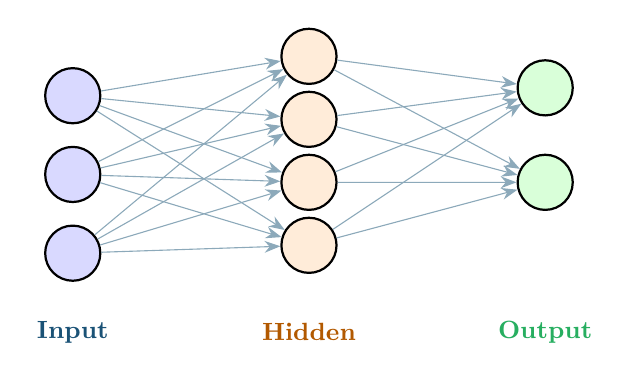
\begin{tikzpicture}[
  neuron/.style={circle, draw, thick, fill=#1, minimum size=0.7cm},
  arr/.style={-{Stealth[length=2mm]}, primary!50}
]
  \foreach \i in {1,2,3} {\node[neuron=blue!15] (i\i) at (0,-\i) {};}
  \foreach \i in {1,2,3,4} {\node[neuron=orange!15] (h\i) at (3,-\i*0.8+0.3) {};}
  \foreach \i in {1,2} {\node[neuron=green!15] (o\i) at (6,-\i*1.2+0.3) {};}
  \foreach \i in {1,2,3} {\foreach \j in {1,2,3,4} {\draw[arr] (i\i) -- (h\j);}}
  \foreach \i in {1,2,3,4} {\foreach \j in {1,2} {\draw[arr] (h\i) -- (o\j);}}
  \node[font=\small\bfseries, primary] at (0,-4) {Input};
  \node[font=\small\bfseries, orange!70!black] at (3,-4) {Hidden};
  \node[font=\small\bfseries, greenhl] at (6,-4) {Output};
\end{tikzpicture}
\end{center}

\begin{itemize}[leftmargin=*]
  \item \textbf{Activation Function:} Introduces non-linearity (e.g., ReLU, Sigmoid, Softmax) so networks can learn complex patterns.
  \item \textbf{Backpropagation:} The algorithm that computes gradients and updates weights to minimize error.
  \item \textbf{Deep Learning:} Neural networks with many hidden layers, powering modern image recognition (CNNs) and language models (Transformers).
\end{itemize}

\subsection{The Perceptron: A Single Neuron}
\begin{definitionbox}[Perceptron]
The simplest neural unit computes a weighted sum of inputs, adds a bias, and passes the result through an activation function:
$$
z=\sum_{i=1}^n w_i x_i + b, \qquad \hat{y}=f(z)
$$
where $f$ is an activation function such as a step function or sigmoid.
\end{definitionbox}

\subsection{Convolutional Neural Networks (CNNs)}
\begin{conceptbox}[How CNNs Process Images]
CNNs use small filters (kernels) that slide over the image to detect local patterns like edges and textures.
\end{conceptbox}
\begin{itemize}[leftmargin=*]
  \item \textbf{Convolution Layer:} Slides a filter over the input, computing dot products to produce a \textbf{feature map} that highlights specific patterns.
  \item \textbf{Pooling Layer (e.g., Max Pooling):} Downsamples feature maps, keeping the strongest signal in each region and reducing computation.
  \item \textbf{Fully Connected Layer:} Combines extracted features to make the final classification decision.
\end{itemize}

\subsection{Recurrent Neural Networks (RNNs) and LSTMs}
\begin{itemize}[leftmargin=*]
  \item \textbf{RNN:} Processes sequential data (text, time series) by feeding the output of each step back as input to the next, maintaining a ``memory'' of previous steps.
  \item \textbf{Vanishing Gradient Problem:} Standard RNNs struggle to learn long-range dependencies because gradients shrink over many steps.
  \item \textbf{LSTM (Long Short-Term Memory):} A specialized RNN with gates (input, forget, output) that control what information to keep or discard, better handling long sequences.
\end{itemize}

%=============================================================
\section{Natural Language Processing and Computer Vision}
%=============================================================

\subsection{Natural Language Processing (NLP)}
\begin{definitionbox}[NLP]
NLP enables computers to understand, interpret, and generate human language, powering chatbots, translation, sentiment analysis, and large language models like GPT.
\end{definitionbox}
\begin{itemize}[leftmargin=*]
  \item \textbf{Tokenization:} Splitting text into words or sub-words for processing.
  \item \textbf{Stopword Removal \& Stemming/Lemmatization:} Removing common low-information words (``the'', ``is'') and reducing words to their root form (``running'' $\to$ ``run'').
  \item \textbf{Part-of-Speech (POS) Tagging:} Labeling each word with its grammatical role (noun, verb, adjective).
  \item \textbf{N-grams:} Contiguous sequences of $n$ words (e.g., bigrams, trigrams) used to capture local word context.
  \item \textbf{Word Embeddings:} Dense vector representations of words (e.g., Word2Vec, GloVe) that capture meaning, so similar words have similar vectors.
  \item \textbf{Attention and Transformers:} The attention mechanism lets a model weigh which words matter most to each other, forming the basis of Transformer models used in modern LLMs.
  \item \textbf{Sentiment Analysis:} Determining whether text expresses positive, negative, or neutral opinion.
  \item \textbf{Large Language Models (LLMs):} Transformer-based models trained on massive text corpora to generate and understand language (e.g., ChatGPT).
\end{itemize}

\subsection{Computer Vision}
\begin{definitionbox}[Computer Vision]
Computer vision enables machines to interpret and understand visual information from images and video, used in face recognition, medical imaging, and self-driving cars.
\end{definitionbox}
\begin{itemize}[leftmargin=*]
  \item \textbf{Image Classification:} Assigning a label to an entire image (e.g., cat vs. dog).
  \item \textbf{Object Detection:} Identifying and locating multiple objects within an image.
  \item \textbf{Image Segmentation:} Labeling every pixel of an image according to the object it belongs to.
  \item \textbf{Convolutional Neural Networks (CNNs):} The dominant deep learning architecture for vision tasks, using the convolution and pooling layers introduced in the Neural Networks section.
\end{itemize}

\begin{examplebox}[Worked Example: One Convolution Step]
A $3\times3$ image region:
$$
\begin{pmatrix}1 & 2 & 0\\ 0 & 1 & 2\\ 1 & 0 & 1\end{pmatrix}
$$
convolved with a $3\times3$ filter of all 1's produces a single output value equal to the sum of all 9 pixels: $1+2+0+0+1+2+1+0+1=8$. Sliding this filter across the full image produces a complete feature map.
\end{examplebox}

%=============================================================
\section{Applications of AI}
%=============================================================

\rowcolors{2}{white}{defbg}
\begin{longtable}{@{}p{3.5cm}p{10cm}@{}}
\toprule
\rowcolor{primary!15}
\textbf{Domain} & \textbf{Example Applications} \\
\midrule
\endhead
Healthcare & Disease diagnosis, medical imaging analysis, drug discovery. \\
\addlinespace
Finance & Fraud detection, algorithmic trading, credit scoring. \\
\addlinespace
Transportation & Self-driving cars, traffic prediction, route optimization. \\
\addlinespace
Business \& IT & Chatbots, recommendation systems, process automation. \\
\addlinespace
Education & Personalized learning, automated grading, tutoring systems. \\
\bottomrule
\end{longtable}

%=============================================================
\section{Ethical and Responsible AI}
%=============================================================

\begin{alertbox}[Key Concerns]
As future IT professionals, you must consider the risks and responsibilities of deploying AI systems.
\end{alertbox}

\begin{itemize}[leftmargin=*]
  \item \textbf{Bias and Fairness:} Models can inherit or amplify biases present in training data.
  \item \textbf{Privacy:} AI systems often require large amounts of personal data, raising data protection concerns.
  \item \textbf{Transparency and Explainability:} Complex models (``black boxes'') can be difficult to interpret or justify.
  \item \textbf{Accountability:} Determining responsibility when an AI system makes a harmful or incorrect decision.
  \item \textbf{Job Displacement:} Automation may replace certain human roles, requiring workforce reskilling.
\end{itemize}

\begin{conceptbox}[Responsible AI Principles]
Fairness $\bullet$ Reliability and Safety $\bullet$ Privacy and Security $\bullet$ Inclusiveness $\bullet$ Transparency $\bullet$ Accountability.
\end{conceptbox}

%=============================================================
\section{Core Mathematical Foundations for AI}
%=============================================================

\subsection{Linear Algebra Essentials}
\begin{itemize}[leftmargin=*]
  \item \textbf{Vector:} Ordered list of numbers, e.g., $\mathbf{x}=[x_1,x_2,\dots,x_n]$.
  \item \textbf{Matrix:} 2D array used to represent datasets and transformations.
  \item \textbf{Dot Product:} $\mathbf{w}\cdot\mathbf{x}=\sum_i w_i x_i$, central in linear models and neural networks.
\end{itemize}

\subsection{Probability Essentials}
\begin{itemize}[leftmargin=*]
  \item \textbf{Conditional Probability:} $P(A|B)=\frac{P(A\cap B)}{P(B)}$.
  \item \textbf{Bayes' Theorem:} 
  $$
  P(A|B)=\frac{P(B|A)P(A)}{P(B)}
  $$
  \item Used in Naive Bayes classifiers, medical diagnosis, and uncertainty-aware AI decisions.
\end{itemize}

\subsection{Optimization Essentials}
\begin{itemize}[leftmargin=*]
  \item Training aims to minimize a loss function $L(\theta)$ over model parameters $\theta$.
  \item Gradient descent update rule:
  $$
  \theta_{t+1}=\theta_t-\eta\nabla L(\theta_t)
  $$
  where $\eta$ is the learning rate.
\end{itemize}

%=============================================================
\section{Exam-Oriented Worked Examples}
%=============================================================

\begin{examplebox}[Worked Example 1: Confusion Matrix]
A classifier gives: $TP=45, TN=40, FP=10, FN=5$.
\begin{itemize}[leftmargin=*]
  \item Accuracy $=\frac{45+40}{100}=0.85=85\%$
  \item Precision $=\frac{45}{45+10}=0.818=81.8\%$
  \item Recall $=\frac{45}{45+5}=0.90=90\%$
  \item F1 $=2\cdot\frac{0.818\cdot0.90}{0.818+0.90}\approx0.857=85.7\%$
\end{itemize}
Interpretation: strong recall means most positives are detected; moderate FP reduces precision.
\end{examplebox}

\begin{examplebox}[Worked Example 2: Entropy and Information Gain]
Consider dataset $S$ with 8 samples: 4 positive and 4 negative.
$$
H(S)=-\frac{4}{8}\log_2\frac{4}{8}-\frac{4}{8}\log_2\frac{4}{8}=1
$$
If attribute $A$ splits into subsets with weighted entropy $0.5$, then:
$$
IG(S,A)=H(S)-0.5=0.5
$$
Higher information gain indicates a better split in decision trees.
\end{examplebox}

\begin{examplebox}[Worked Example 3: One Gradient Descent Step]
For loss $L(w)=(w-3)^2$, gradient is $\nabla L=2(w-3)$. If $w_0=0$ and learning rate $\eta=0.1$:
$$
\nabla L(w_0)=2(0-3)=-6
$$
$$
w_1=w_0-\eta\nabla L=0-0.1(-6)=0.6
$$
The parameter moves toward the optimum $w=3$.
\end{examplebox}

\begin{examplebox}[Worked Example 4: Naive Bayes Classification]
Predict whether to ``Play'' tennis given \textit{Outlook = Sunny}, using training statistics $P(\text{Play})=0.6$, $P(\text{Sunny}|\text{Play})=0.33$, $P(\text{No Play})=0.4$, $P(\text{Sunny}|\text{No Play})=0.5$:
$$
P(\text{Play}|\text{Sunny}) \propto 0.6 \times 0.33 = 0.198
$$
$$
P(\text{No Play}|\text{Sunny}) \propto 0.4 \times 0.5 = 0.200
$$
Since $0.200 > 0.198$, Naive Bayes predicts \textbf{No Play} (the two scores are close, showing how sensitive the method is to the input statistics).
\end{examplebox}

\begin{examplebox}[Worked Example 5: K-Nearest Neighbors]
A new point has distances to 5 labeled neighbors: $1.2\,(A), 2.0\,(A), 2.5\,(B), 3.0\,(B), 3.1\,(B)$. For $k=3$, the three nearest neighbors are $1.2(A), 2.0(A), 2.5(B)$. Majority class $=A$ (2 votes vs.\ 1), so the new point is classified as \textbf{A}.
\end{examplebox}

\begin{examplebox}[Worked Example 6: One Iteration of K-Means]
Points $\{2,4,10,12\}$ with initial centroids $c_1=3, c_2=11$.
\begin{itemize}[leftmargin=*]
  \item Assign: $2\to c_1$, $4\to c_1$ (closer to 3), $10\to c_2$, $12\to c_2$ (closer to 11).
  \item Update centroids: $c_1=\frac{2+4}{2}=3$, $c_2=\frac{10+12}{2}=11$.
\end{itemize}
Centroids are unchanged, so the algorithm has already \textbf{converged}.
\end{examplebox}

\begin{examplebox}[Worked Example 7: Genetic Algorithm --- One Generation]
Parent chromosomes (bit strings): $P_1=11001$, $P_2=10011$. Single-point crossover after position 2:
\begin{itemize}[leftmargin=*]
  \item Child $C_1 = \underbrace{11}_{\text{from }P_1} + \underbrace{011}_{\text{from }P_2} = 11011$
  \item Child $C_2 = \underbrace{10}_{\text{from }P_2} + \underbrace{001}_{\text{from }P_1} = 10001$
\end{itemize}
Mutation (flip last bit of $C_1$ with small probability): $11011 \to 11010$. These children form the next generation.
\end{examplebox}

\begin{examplebox}[Worked Example 8: One Q-Learning Update]
Given $Q(s,a)=2$, reward $r=1$, learning rate $\alpha=0.5$, discount $\gamma=0.9$, and $\max_{a'}Q(s',a')=3$:
$$
Q(s,a) \leftarrow 2 + 0.5\big[1 + 0.9(3) - 2\big] = 2 + 0.5(1.7) = 2.85
$$
The Q-value increases from 2 to 2.85, reflecting a better-than-expected outcome.
\end{examplebox}

%=============================================================
\section{Quick Revision Glossary}
%=============================================================

\rowcolors{2}{white}{defbg}
\begin{longtable}{@{}p{3.3cm}p{10.2cm}@{}}
\toprule
\rowcolor{primary!15}
\textbf{Term} & \textbf{One-Line Meaning} \\
\midrule
\endhead
Agent & Entity that perceives via sensors and acts via actuators to achieve goals. \\
\addlinespace
PEAS & Performance, Environment, Actuators, Sensors --- framework for describing a task environment. \\
\addlinespace
Heuristic $h(n)$ & Estimated cost from node $n$ to the goal, used to guide informed search. \\
\addlinespace
Admissible Heuristic & A heuristic that never overestimates the true cost to the goal. \\
\addlinespace
Minimax & Game-tree search where MAX maximizes and MIN minimizes the backed-up value. \\
\addlinespace
Alpha-Beta Pruning & Skips branches in minimax that cannot affect the final decision. \\
\addlinespace
CSP & Problem defined by variables, domains, and constraints; solved via backtracking. \\
\addlinespace
Planning / STRIPS & Finding an action sequence to reach a goal using preconditions, add lists, and delete lists. \\
\addlinespace
Iterative Deepening & Repeated DFS with increasing depth limits; combines BFS and DFS advantages. \\
\addlinespace
Semantic Network & Graph representation of concepts and their relationships. \\
\addlinespace
Forward Chaining & Data-driven inference: facts $\to$ rules $\to$ new facts $\to$ goal. \\
\addlinespace
Backward Chaining & Goal-driven inference: start from the goal and verify supporting facts. \\
\addlinespace
Fuzzy Logic & Reasoning with partial truth values (0 to 1) instead of strict true/false. \\
\addlinespace
Overfitting & Model fits training data (including noise) too closely and generalizes poorly. \\
\addlinespace
Underfitting & Model is too simple to capture the underlying pattern in the data. \\
\addlinespace
Precision & $TP/(TP+FP)$ --- how many predicted positives were actually correct. \\
\addlinespace
Recall & $TP/(TP+FN)$ --- how many actual positives were correctly found. \\
\addlinespace
Entropy & Measure of impurity/disorder in a dataset; used to build decision trees. \\
\addlinespace
Information Gain & Reduction in entropy achieved by splitting on a given attribute. \\
\addlinespace
Gradient Descent & Iterative optimization that updates parameters opposite to the loss gradient. \\
\addlinespace
Perceptron & Simplest neural unit computing a weighted sum plus bias through an activation function. \\
\addlinespace
CNN & Neural network using convolution/pooling layers, dominant for image tasks. \\
\addlinespace
RNN / LSTM & Neural networks for sequential data; LSTM adds gates to retain long-term memory. \\
\addlinespace
Word Embedding & Dense vector representation of a word capturing semantic meaning. \\
\addlinespace
K-Means & Unsupervised algorithm that groups data into $k$ clusters via iterative centroid updates. \\
\addlinespace
KNN & Classifies a point by majority vote among its $k$ nearest labeled neighbors. \\
\addlinespace
MDP & Formalizes RL via states, actions, transition probabilities, rewards, and a discount factor. \\
\addlinespace
Policy & A strategy $\pi(s)$ mapping states to the actions an agent should take. \\
\addlinespace
Q-Learning & Model-free RL algorithm that learns action values directly from experience. \\
\addlinespace
Exploration vs.\ Exploitation & Trade-off between trying new actions and using the best-known action. \\
\bottomrule
\end{longtable}

%=============================================================
\section{Question Bank Blueprint (80 Marks Support)}
%=============================================================

\begin{conceptbox}[Suggested 80 Marks Distribution]
\begin{itemize}[leftmargin=*]
  \item \textbf{Section A:} MCQs and definitions (20 marks)
  \item \textbf{Section B:} Short conceptual questions (20 marks)
  \item \textbf{Section C:} Descriptive/theory questions (20 marks)
  \item \textbf{Section D:} Numerical/problem-solving questions (20 marks)
\end{itemize}
\end{conceptbox}

\subsection{Important Theory Questions}
\begin{itemize}[leftmargin=*]
  \item Differentiate symbolic AI, machine learning, and deep learning with examples.
  \item Explain and compare simple reflex, goal-based, and utility-based agents.
  \item Explain BFS, DFS, and A* with completeness and optimality.
  \item Describe PEAS with one real-world agent design.
  \item Explain the Minimax algorithm and how Alpha-Beta pruning improves it.
  \item Define a CSP and describe backtracking search with an example.
  \item Explain STRIPS-style planning and differentiate forward and backward planning.
  \item Differentiate forward chaining and backward chaining with an example each.
  \item Explain fuzzy logic and why it is useful for real-world control systems.
  \item Compare supervised, unsupervised, and reinforcement learning with examples.
  \item Define an MDP and explain the Q-learning update rule.
  \item Explain the exploration-exploitation trade-off in reinforcement learning.
  \item Explain overfitting, underfitting, and the bias-variance tradeoff.
  \item Describe how a CNN processes an image, mentioning convolution and pooling.
  \item Explain the difference between RNNs and LSTMs and why LSTMs help with long sequences.
  \item Discuss ethical issues in AI and practical mitigation methods.
\end{itemize}

\subsection{Important Numerical/Analytical Questions}
\begin{itemize}[leftmargin=*]
  \item Compute accuracy, precision, recall, and F1 from a confusion matrix.
  \item Solve one A* search expansion step given $g(n)$ and $h(n)$ values.
  \item Compute the backed-up values of a small minimax tree.
  \item Solve a 3-region map-coloring CSP by hand using backtracking.
  \item Construct a simple STRIPS plan given actions with preconditions and effects.
  \item Compute entropy and information gain for a small dataset split.
  \item Classify a test instance using Naive Bayes given simple probability tables.
  \item Classify a new point using KNN given distances to labeled neighbors.
  \item Perform one iteration of K-Means clustering given points and initial centroids.
  \item Perform one generation (crossover and mutation) of a genetic algorithm.
  \item Perform one Q-learning update given $Q(s,a)$, reward, learning rate, and discount factor.
  \item Perform one gradient descent update for a simple loss function.
\end{itemize}

\subsection{Sample MCQs with Answer Key}
\begin{enumerate}[leftmargin=*]
  \item Which search strategy is guaranteed to find the shallowest solution?\\
  (a) DFS \quad (b) BFS \quad (c) Greedy Best-First \quad (d) Hill Climbing
  \item In Minimax, which player minimizes the backed-up value?\\
  (a) MAX \quad (b) MIN \quad (c) Both \quad (d) Neither
  \item Alpha-beta pruning skips a branch when:\\
  (a) $\alpha < \beta$ \quad (b) $\alpha \geq \beta$ \quad (c) $\alpha = 0$ \quad (d) $\beta = 1$
  \item Which metric is most reliable for a highly imbalanced dataset?\\
  (a) Accuracy \quad (b) F1-score \quad (c) Raw error count \quad (d) None
  \item Which learning type uses labeled data?\\
  (a) Unsupervised \quad (b) Reinforcement \quad (c) Supervised \quad (d) Fuzzy
  \item CNNs are primarily used for:\\
  (a) Tabular data \quad (b) Image data \quad (c) Audio only \quad (d) Text only
  \item Backward chaining is best described as:\\
  (a) Data-driven \quad (b) Goal-driven \quad (c) Random \quad (d) Exhaustive only
  \item In Q-learning, the term $\max_{a'}Q(s',a')$ represents:\\
  (a) The immediate reward \quad (b) The best estimated future value \quad (c) The learning rate \quad (d) The discount factor
  \item STRIPS actions are defined using:\\
  (a) Weights and biases \quad (b) Preconditions and effects \quad (c) Kernels and filters \quad (d) Support vectors
\end{enumerate}
\begin{conceptbox}[Answer Key]
1--(b), 2--(b), 3--(b), 4--(b), 5--(c), 6--(b), 7--(b), 8--(b), 9--(b)
\end{conceptbox}

%=============================================================
\section{Summary}
%=============================================================

\begin{examplebox}[Expanded Key Takeaways]
\begin{itemize}[leftmargin=*]
  \item AI combines reasoning, search, knowledge representation, and learning to build intelligent behavior.
  \item Agent design and search strategies (including adversarial search, CSPs, and planning) are central to classic AI problem solving.
  \item Knowledge representation, chaining, and uncertainty handling (Bayesian networks, fuzzy logic) let systems reason under real-world conditions.
  \item Machine learning, reinforcement learning, and deep learning provide data-driven and reward-driven intelligence, from classic algorithms (Naive Bayes, KNN, K-Means, Q-learning) to CNNs, RNNs, and Transformers.
  \item Evaluation metrics, probability, and basic mathematics are essential for exam success and practical model validation.
  \item Responsible AI principles must guide all stages of system design and deployment.
\end{itemize}
\end{examplebox}

\end{document}
